\section*{Hard Disk Drives Interface}
\begin{itemize}
\item consists of a large number of sectors (512-byte blocks): numbered from 0 to $n-1$ on a disk with $n$ sectors; each can be read and written
\item can be viewed as \texttt{array[n]} of sectors: 0 to $n-1$ (\textbf{address space})
\item OS typically read or write $\geq$ 4KB at a time; Hardware only guarantees a single 512-byte write is \textbf{atomic}
\item if untimely power loss occurs $\to$ only a portion of a large write may complete (aka \textbf{torn write})
\end{itemize}
\section*{Modern Disk Components (Basic Geometry)}
\begin{itemize}
\item \textbf{platter} a circular hard surface on which data is stored persistenly by inducing magnetic changes to it
  \begin{itemize}
  \item a disk may have $\geq$ 1 platter; each has 2 sides (called surface)
  \item platters usually made of hard material (aluminum), coated with thin magnetic layer to persistently store bits even when drive's powered off
  \end{itemize}
\item platters all bound to \textbf{spindle}, which is connected to motor that spins platters around (when powered on) at a constant/fixed rate
  \begin{itemize}
  \item The rotation rate often measured in rotations per minute (RPM), and typical modern values:  7,200 - 15,000 RPM
  \item often interested in the time of a single rotation: 10,000 RPM $\to$ a single rotation takes about 6ms (see right equations)
  \end{itemize}
\item Data is encoded on each surface in concentric circles of sectors (each such such concentric circle is called \textsc{track})
  \begin{itemize}
  \item A single surface contains thousands of tracks, tightly packed together
  \item hundreds of tracks fitting into the width of a human hair
  \end{itemize}
\item To read/write from the surface, need a mechanism to either sense (read) the magnetic patterns on the disk or to induce a change in (write) them
  \begin{itemize}
  \item This process of reading and writing is accomplished by the \textbf{disk head}
  \item there is one such head per surface of the drive
  \item The disk head is attached to a single \textbf{disk arm}; it moves across the surface to position the head over the desired track
  \end{itemize}
\end{itemize}
\begin{minipage}{.35\linewidth}
  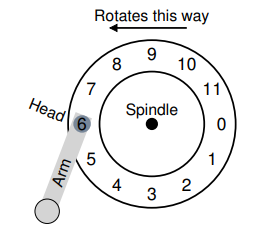
\includegraphics[width=\linewidth,height=3cm]{imgs/disk_stah}
\end{minipage}
\begin{minipage}{.65\linewidth}
  \flushleft
  \begin{itemize}
  \item must wait for desired sector to rotate under disk header; happens often in modern drives
  \item wait $\to$ key component of I/O service time, named \mb{rotational delay} (aka rotation delay)
  \item if full rotational delay is $R \to$ needs $\frac{R}{2}$ if stay at 6 and wait for 0 for read/write
  \item worse case: stay at 6 and wait for 5 $\to$ need full rotational delay $R$
  \end{itemize}
\end{minipage}
\begin{minipage}{.75\linewidth}
  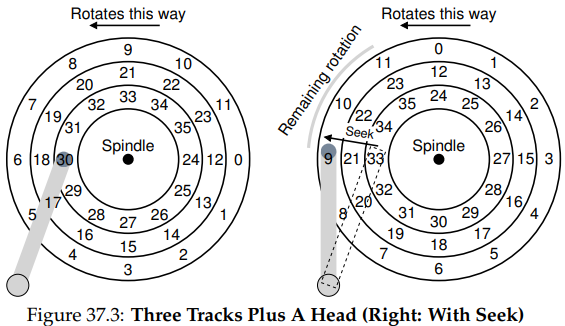
\includegraphics[width=\linewidth]{imgs/disk_3tracks}
\end{minipage}
\begin{minipage}{.25\linewidth}
  \flushleft
  \begin{itemize}
  \item head currently positioned over innermost track
  \item \mo{innermost} track: sectors 24-35
  \item \mo{middle} track: sectors 12-23
  \item \mo{outermost} track: sectors 0-11
  \item request a read to sector 11
  \item steps shown $\downarrow$
  \end{itemize}
\end{minipage}
\begin{enumerate}
\item drive moves disk arm to correct track (outermost) in a process (\mb{seek})
\item \textbf{seek} (one of most costly disk ops) has many phases
  \begin{itemize}[leftmargin=.1em]
  \item \emph{acceleration}: disk arm gets moving
  \item \emph{coasting} disk arm moves at full speed
  \item \emph{deceleration} disk arm slows down at full speed
  \item \emph{settling} disk head positioned over correct track: $T_{\text{settling}} = 0.5 \sim 2$ms
  \end{itemize}
\item[] during the seek, platter has rotated, in this case about 3 sectors. Thus, sector 9 is just about to pass under disk head, and we must only endure a short rotational delay to complete the transfer
\item \textbf{transfer}: sector 11 passes under disk head and data read/written to/from the surface; usually $T_{\text{transfer}} < T_{\text{seek}}$ and $T_{\text{transfer}} < T_{\text{rotation}}$
\end{enumerate}
\begin{minipage}{.45\linewidth}
  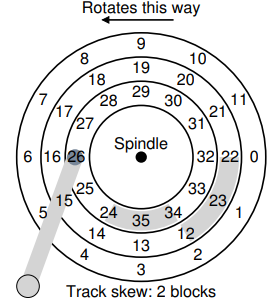
\includegraphics[width=\linewidth]{imgs/disk_trackskew}
\end{minipage}
\begin{minipage}{.55\linewidth}
  \flushleft
  \begin{itemize}
  \item \mb{track skew} rearrange sectors to ensure sequential reads to be properly served even when crossing track boundaries
  \item w/t skew, head would be moved to next track but the desired next block would've already rotated under head $\to$ wait almost full rotational delay
  \item outer tracks have more space $\to$ more sectors (\mo{multi-zoned} disk drives)
  \item \mb{cache} (track buffer) t some small amount of memory (usually around 8 or 16 MB) which drive uses to hold data read from or written to disk
  \item \mb{write back} data $\to$ cache
  \item \mb{write through} data $\to$ disk
  \end{itemize}
\end{minipage}
\begin{itemize}
\item Write back somets makes drive appear ``faster'', but can be dangerous
\item  if file sys/apps require that data be written to disk in certain order for correctness, write-back caching can lead to problems (see journaling)
\item 10K RPM disk, each rotation takes ? milliseconds (1)
\item 100 MB/second disk, to transfer 512 KB block in ? milliseconds (2)
\end{itemize}
\[
  \frac{Time(ms)}{1\;Rot.} = \frac{1\;\cancel{minute}}{10,000\;Rot.}\cdot \frac{60\; \cancel{second}}{1\;\cancel{minute}}\cdot \frac{1000\;ms}{1\;\cancel{second}} = \frac{60,000\;ms}{10,000\;Rot.} = \frac{6\;ms}{Rotation}
\]
\[
  \frac{Time(ms)}{1\;Request.} = \frac{512\;\cancel{KB}}{1\;Request}\cdot \frac{1\;\cancel{MB}}{1024\;\cancel{KB}}\cdot \frac{1\;\cancel{second}}{100\;\cancel{MB}}\cdot \frac{1000\;ms}{1\;\cancel{second}} = \frac{5\;ms}{Request}
\]
\section*{I/O Time Calculation}
\begin{itemize}
\item average I/O time calculation: $T_{I/O} = T_{seek} + T_{rotation} + T_{transfer}$
\item average time of data transfer: $R_{I/O} = \frac{Size_{transfer}}{T_{I/O}}$
\item \textbf{random}: read/write small (4KB) to random locations on disk (DBMS)
\item \textbf{sequential}: read/write a large number of consecutive sectors from disk
\item Cheetah: ``high performance'' drive market, spin as fast as possible, low seek times, and transfer data quickly
\item Barracuda: ``capacity'' market, cost per byte matters most $\to$ slower but pack as many bits as possible into the space available
\end{itemize}
\begin{minipage}{.5\linewidth}
  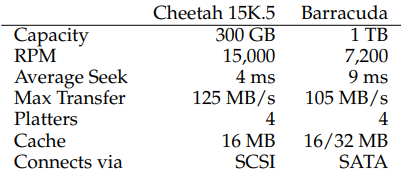
\includegraphics[width=\linewidth]{imgs/disk_scsivssata}
\end{minipage}
\begin{minipage}{.5\linewidth}
  \flushleft
  \begin{itemize}
  \item $T_{trans-Ch} = \frac{4KB}{125MB/s} \approx 32\; \mu\text{s}$
  \item $T_{trans-Ba} = \frac{4KB}{105MB/s} \approx 38\; \mu\text{s}$
  \item $1\;\text{ms} = 1000\; \mu\text{s}$
  \end{itemize}
  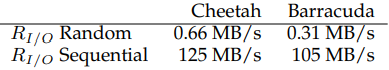
\includegraphics[width=\linewidth]{imgs/disk_scsivssata1}
\end{minipage}
\begin{enumerate}
\item there is a huge gap in drive performance between random and sequential workloads: $\approx 200$ for the Cheetah and $\approx 300+$ for Barracuda
\item there is a large difference in performance between high-end ``performance'' drives (expensive) and low-end ``capacity'' drives (cheap)
\end{enumerate}
\begin{tcolorbox}[left=0mm, top=1mm, right=0mm, rightlower=0mm, bottom=1mm,
  title= Use Disks Sequentially,
  halign title=center]
  When at all possible, transfer data to/from disks in a sequential manner. If that is not possible, at least try to transfer data
in large chunks: the bigger, the better. If I/O is done in little random
pieces, I/O performance will suffer dramatically. Also, users will suffer.
\end{tcolorbox}
\begin{itemize}
\item Scheduling algorithms for CPU time are also useful for I/O
\end{itemize}
\section*{Disk Scheduling: shortest job first (SJF principle)}
\begin{itemize}
\item disk scheduler can estimate seek and rotational delay of a disk request
\item (greedily) pick the one that will take the least time to service first
\end{itemize}
\begin{minipage}{.25\linewidth}
  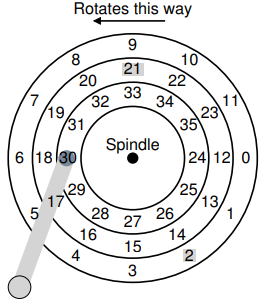
\includegraphics[width=\linewidth]{imgs/disk_sstf}
\end{minipage}
\begin{minipage}{.75\linewidth}
  \flushleft
  \begin{itemize}
  \item shortest-seek-(time)-first (SS(T)F) orders queue of I/O requests by track, picking those on the nearest track to complete first
  \item $P_{\text{head}}$ over inner track: request 21[mid] or 2[outer]?
  \item request \textbf{21} first; when it completes; \emph{then} request \textbf{2}
  \item Position of disk head relative to the requested position matters \emph{more}
than length of the transfer
  \end{itemize}
\end{minipage}
\begin{enumerate}
  \item drive geometry (\texttt{array[n]} of sectors) \mr{invisible} to OS $\to$ OS uses \mo{nearest-block-first} (NBF) to sched reqs with nearest block addr next
  \item \mr{starvation}: steady stream of reqs to inner track (current head pos) $\to$ Requests to other tracks be ignored completely due to pure SSTF
\end{enumerate}
\section*{Elevator (SCAN, F-SCAN, C[ircular]-SCAN) $\to$ prevent starvation}
\begin{enumerate}
\item \textbf{SCAN} moves back/forth across disk serving reqs in order across tracks $\to$ passing through middle twice before back to outer again
  \begin{itemize}[leftmargin=.1em]
  \item \mb{sweep} a single pass across disk (outer $\to$ inner or inner $\to$ outer)
  \item requests on already-serviced track in this sweep will be queued until the next sweep (in the other direction)
  \end{itemize}
\item \textbf{F-SCAN} freezes the queue to be serviced when doing a \emph{sweep}
    \begin{itemize}[leftmargin=.1em]
  \item places reqs coming in during the sweep into queue to be served later
  \item avoids starvation of far-away requests, by delaying the servicing of late-arriving (but nearer by) requests
  \end{itemize}
\item \textbf{C-SCAN} only sweeps from outer-to-inner, and then resets at the outer track to begin again $\to$ a bit more fair to inner and outer tracks
\item[] SCAN and its cousins \texttt{!=} the best scheduling tech:
  \begin{enumerate*}[label={\alph*},font={\color{red!50!black}\bfseries}]
  \item not actually adhere as closely to the principle of SJF as they could;
  \item ignore rotation
  \end{enumerate*}
\end{enumerate}
\section*{Shortest Positioning Time First (SPTF)}
\begin{minipage}{.3\linewidth}
  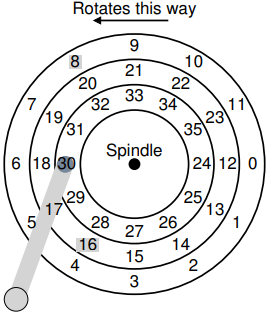
\includegraphics[width=\linewidth]{imgs/disk_sstf1}
\end{minipage}
\begin{minipage}{.7\linewidth}
  \flushleft
  \begin{itemize}
  \item scheduler has to decide: sched \textbf{16} or \textbf{8} for next?
  \item depends on relative time of seeking and rotation
  \item if $T_{\text{seek}} \gg T_{\text{rot.}} \to$ SSTF (or variants) are fine
  \item if $T_{\text{seek}} \ll T_{\text{rot.}} \to$ seek \textbf{further} to service request 8 on outer track \emph{better} than seek to service 16 on middle track (almost full rotation)
  \item On modern drives $T_{\text{seek} \approx T_{\text{rot.}}} \to$ SPTF is useful
  \item OS knows little about track boundaries and disk current head position (in rotational sense), $\to$ SPTF is usually performed inside a drive
  \end{itemize}
\end{minipage}
\begin{itemize}
\item older OS did all the scheduling: check pending requests, pick the best one, issue it to the disk. When that request completed, sched next one
\item modern disk drives have sophisticated internal schedulers (inside disk controller, all relevant details available, including exact $Pos_{\text{head}}$):
  \begin{enumerate}[leftmargin=.2em]
  \item OS scheduler issues what it thinks the best few requests all to disk
  \item disk uses its internal knowledge of $Pos_{\text{head}}$ and detailed track layout info to service said requests in the best possible (SPTF) order
  \item \mb{I/O merging} adjacent reqs on same track (eg 33, 34) will be merged; important at OS level $\because$ requests number to disk $\downarrow \to$ overheads $\downarrow$
  \item immediately issue req to drive (\mo{work-conserving}) $to$ disk never idle
  \item \mo{non-work-conserving}: wait for new/ better req to arrive $\to$ overall efficiency $\uparrow$ (deciding when to wait \& for how long can be tricky)
  \end{enumerate}
\end{itemize}
\section*{Linux Completely Fair Queueing (CFQ) scheduler}
\begin{itemize}
\item queue for each process; yield slice only if idle for given time
\item weighted RR between queues with slice-time proportional to priority
\item CFQ replaced by Budget Fair Queuing (BFQ)
\item other Linux scheduler:
  \begin{enumerate*}[label={\alph*},font={\color{red!50!black}\bfseries}]
  \item \texttt{noop} first come first serve.
  \item \texttt{deadline} impose a ``deadline'' on each I/O req to avoid starvation
  \end{enumerate*}
\end{itemize}
